\section{Approach Adopted}

Grid performance monitoring in this project is examed using {\bf GMA}, an architecture that established to provide the standards for a distributed monitoring system. The technologies that will be discussed here are about the Information Infrastructure that provides the metrics to the users/applications.

The metrics are generated using {\bf Linux kernel}'s load average functions. {\bf Ganglia} is used to take that metrics and synchronize all cluster nodes with the relevant information, over the {\bf multicast channel}.

Nagios is configured using a {\bf custom script} that takes the information for the cluster nodes, and periodically queries the {\bf Gmond} to get the metrics for the discovered nodes. The results are stored in its repository and using RRDTool and pnp4nagios, graph reports are generated on demand.

To pass the information, two different information systems are examined, {\bf BDII and WSRF}. Both are used in modern grid implementations and are described in {\bf MDS specification}. BDII queries event source (Gmond) using Perl/Python LDAP libraries. The results taken, fill the directory schema which has been extended using {\bf Glue schema} specification for Proccessor Load in Computing Element structure.

{\bf MDS4} introduces the use of {\bf WSRF} in grid information system. A {\bf Ganglia Information Provider} using {\bf XSLT} takes the XML output from Gmond and aggregates the metrics using WSRF {\bf Aggregation Framework}. In front of it, a Tomcat instance serves the {\bf WebMDS} frontend to allow {\bf XPath} queries to the results that has been aggregated.

Finally, two sample small applications has been developed to provide a homogeneous interface that display the same information using the two different information systems.

\section{Design Methods}

\subsection{Grid Monitoring Architecture}

By definition \cite{Taylor2006} Grid Monitoring Architecture consists of three components, as shown in Figure \ref{figure:gma}:
\nomenclature{GMA}{Grid Monitoring Architecture}

\begin{enumerate}
\item {\bf Directory Service} which supports the publish and discovery of the information
\item {\bf Producer component}: which is responsible for the availability of the performance data that takes from the event source and
\item {\bf Consumer component}: the one that requests the performance data and receives the metrics from the producer.
\end{enumerate}

\begin{figure}[htb]
\centering
 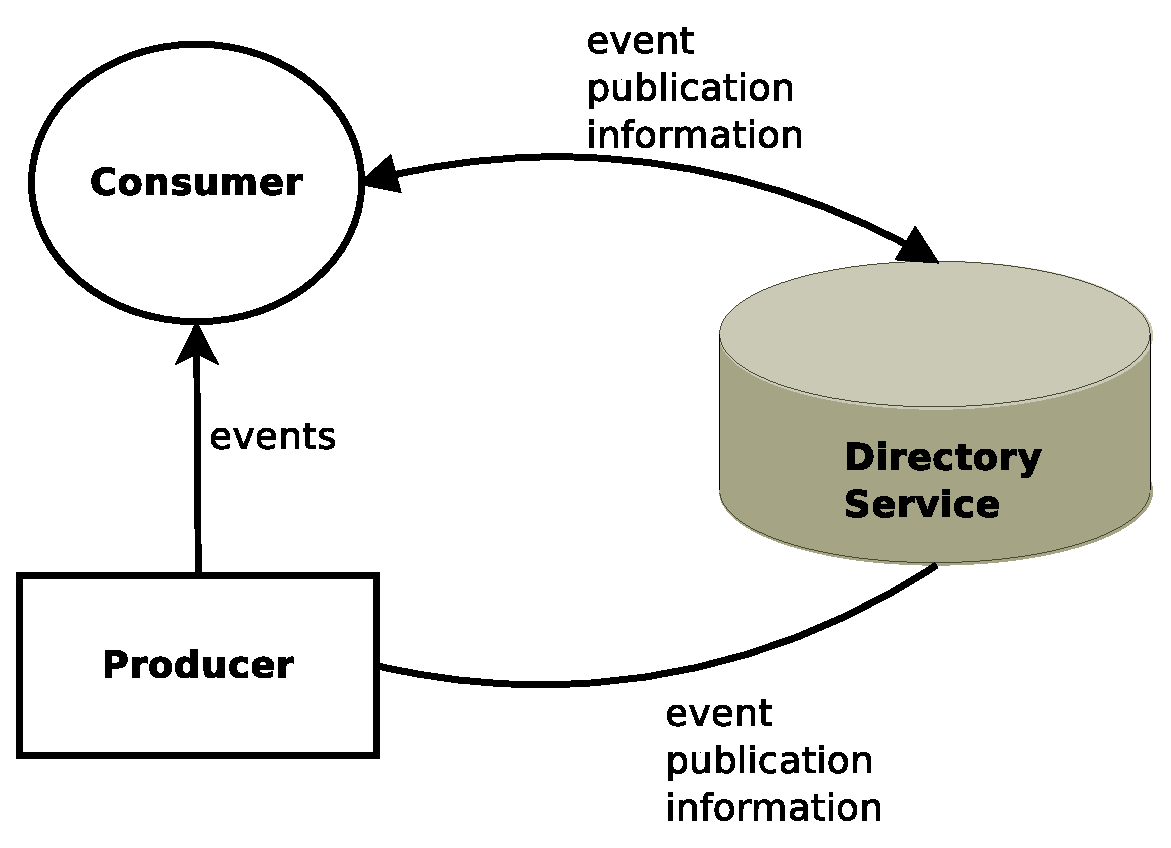
\includegraphics[width=4in]{images/gma.eps}
\caption{Grid Monitoring Architecture}
\label{figure:gma}
\end{figure}

In GMA, all metrics that are transmitted by the producer are handled as events with a timestamp, so performance data should be accurate. These events are transmitted to the consumer directly, and not through the directory service (whose role is just to advertise producers to consumers and vice versa). The GMA recommends that the structure of the data should be following a schema definition. 

Grid Monitoring Architecture supports two models to handle the communication between producers and consumers:

\begin{itemize}
\item {\bf Streaming publish/subscribe model}
\item {\bf Query/Response model}
\end{itemize}

The directory service is used by both producers to discover consumers and consumers to discover producers. The information of the availability of each producer/consumer is published to the directory service, and each component may initiate a connection to another type of component that has discovered in the directory service. Even though the role of the directory service is so centric in the discovery of components between each other, the performance data messages are transfered between the producer/consumer directly and not via the Directory Service.

\subsection{GLUE Schema}
gained wide acceptance given its adoption by Globus MDS3

GLUE schema came to provide the interoperability needed between US and European Physics Grid Projects. As a standard, a common schema was introduced to describe and monitor the grid resources. Major components include:

\begin{itemize}
\item Computing Element (CE)
\item Storage Element (SE)
\item Network Element (NE)
\end{itemize}

The implementation of Glue schema may be using LDAP, XML or SQL. The MDS implementation of the Glue schema in this project includes the core Information Provider and the Ganglia Interface for the cluster information.

\nomenclature{GLUE}{Grid Laboratory Uniform Environment}

\begin{figure}[htb]
\centering
 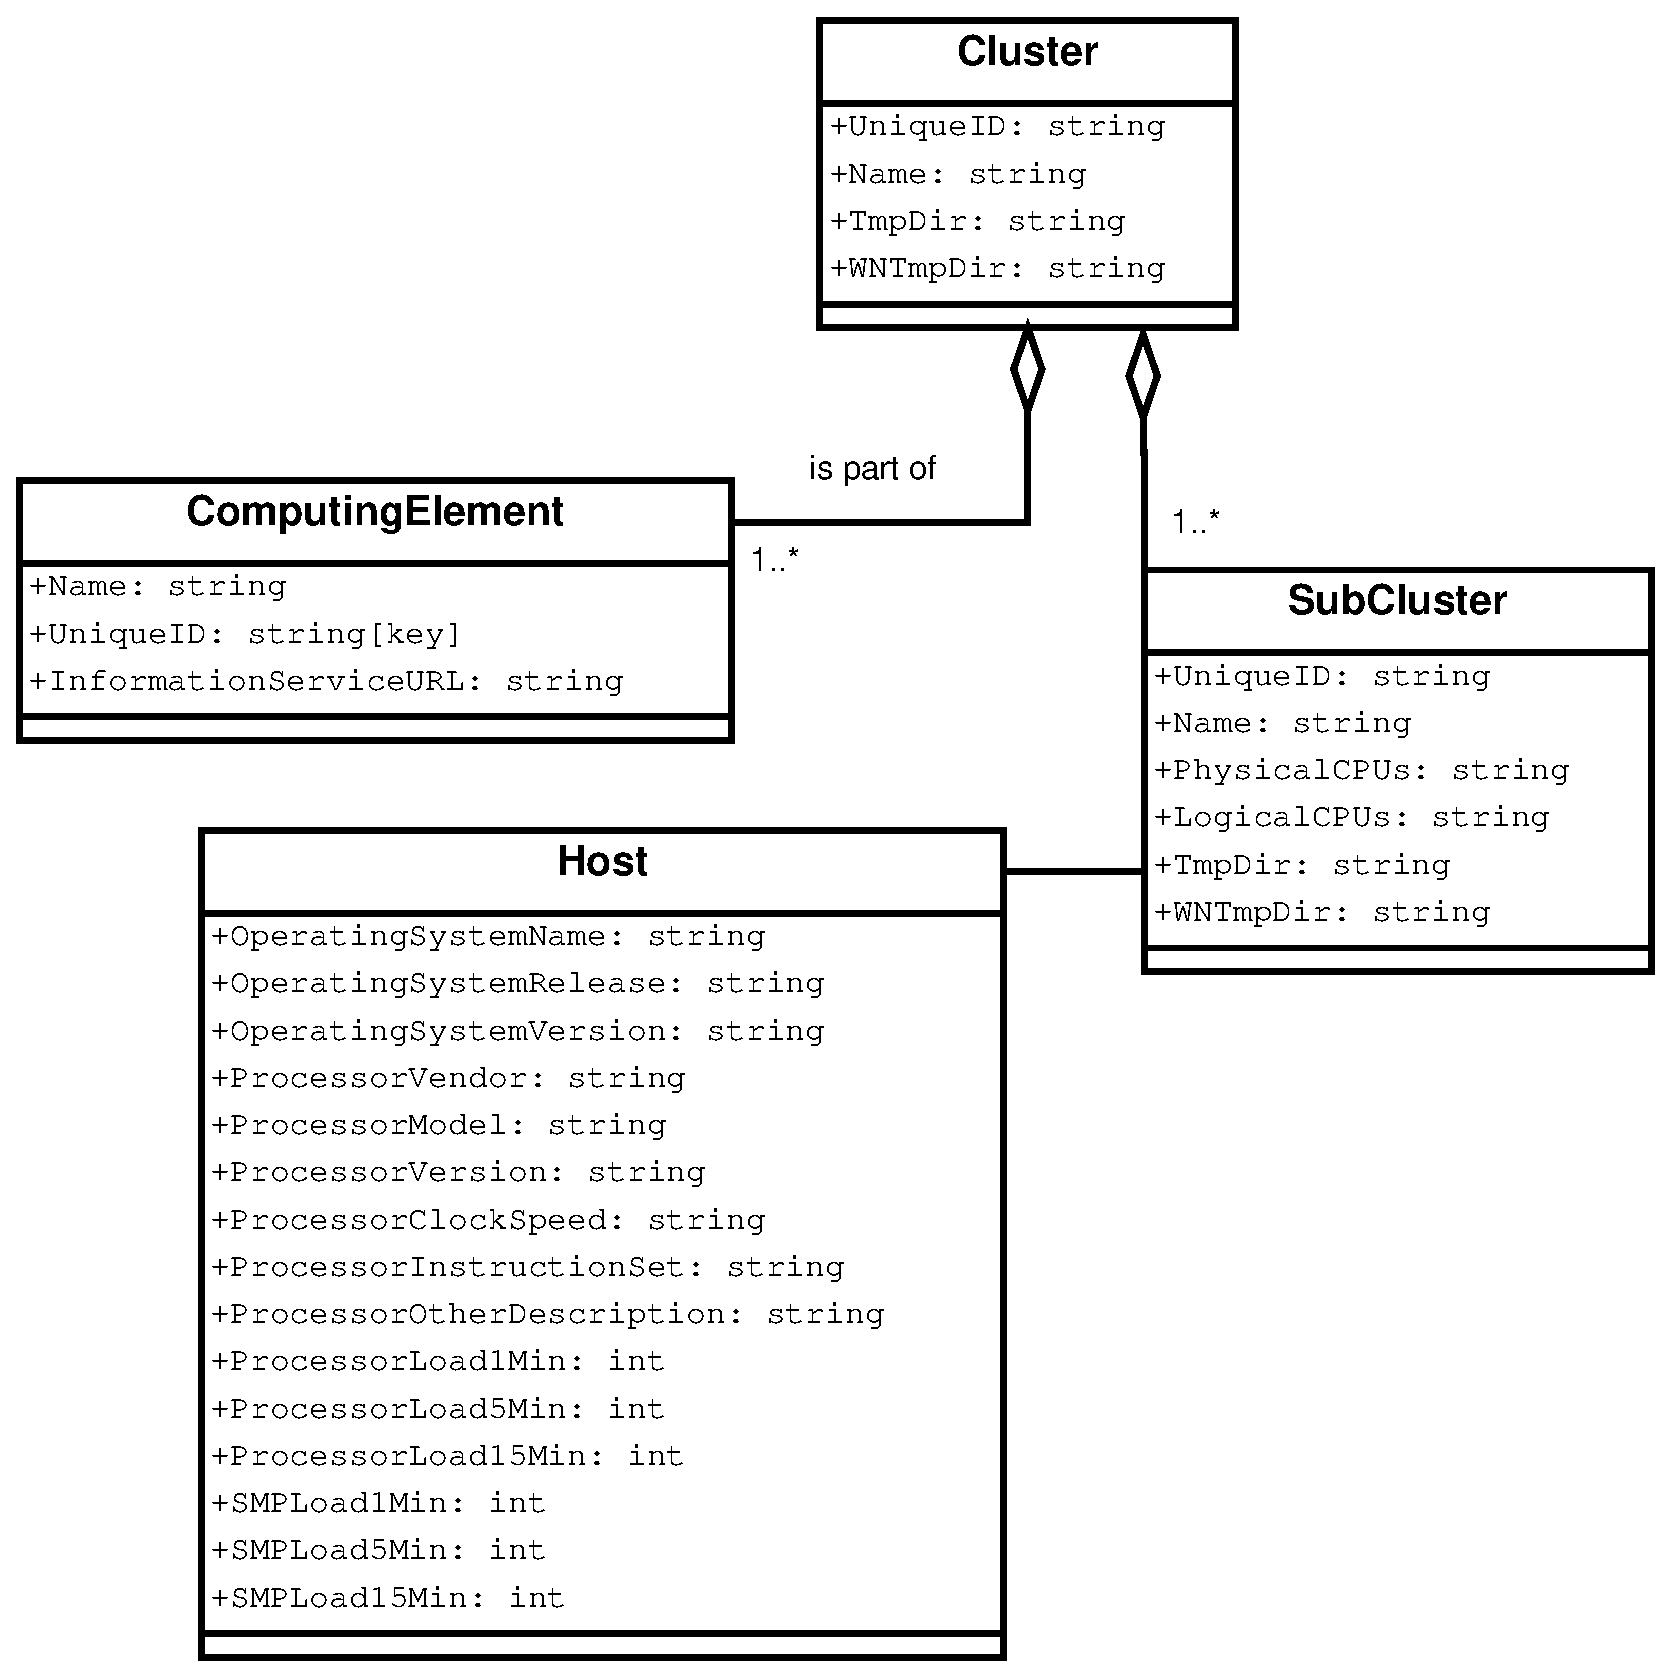
\includegraphics[width=5in]{images/gluece_ext.eps}
\caption{GLUE schema 2.0 extention for Host and SMP Load}
\label{figure:gluece_ext}
\end{figure}


\subsection{Information Infrastructure}

To design the Information Infrastructure for distributed computing applications some requirements have been considered such as performance, scalability, cost and uniformity.

Because grid computing applications usually operate in large scale installations, there are performance requirements for the information infrastructure. It should allow rapid access to configuration information that is frequently used, using {\bf caching to query periodically each host or index server for the metrics}.

The number of components in a grid infrastructure scales up to hundreds of thousands of nodes, and these components should be available for queries by many different tools. That information should be discoverable using information indexes.

Deployments, maintenance and operations in a large installation of many systems has operational costs for human resources. The information system should automaticaly discover and serve the availability paths for applications and grid resources/servives.

Because of the large number of different heterogeneous networks of nodes and clusters, there is a need of uniformity. Uniformity helps to simplify the developers to build applications that give better configuration decisions. APIs for common operations and data models for the representation of that information. Resources are devided in groups of computing, storage, network elements, etc.

The solution proposed by GLUE standard and X.500 (Directory Service) is the key feature to scale, and get uniformity. It may be used to provide extensible distributed directory services. It is optimised for reads, its binary-tree like hierarchy and usually backend data structure provides a framework that well organize the information that need to be delivered by an Information Infrastructure.\cite{mds1}

\section{Data-acquisition Systems}

\subsection{Metrics}\label{subsec:metrics}

{\bf CPU load} is taken using the pseudo /proc/loadavg file which in turn is
filled by Linux kernel's CALC\_LOAD macro. This function takes 3 parameters.
The load-average bucket, a $y$ constant that is calculated using formula
\[
y=\frac{2^{11}}{2^{((5log_2(e))/60x)}}
\]
for values $x=1$, $x=5$ and $x=15$ (where x represent the minutes and y the
exponent constant), and the number of how many processes are in the queue, in
running or uninterruptible state.

\begin{figure}[htb]
\centering
 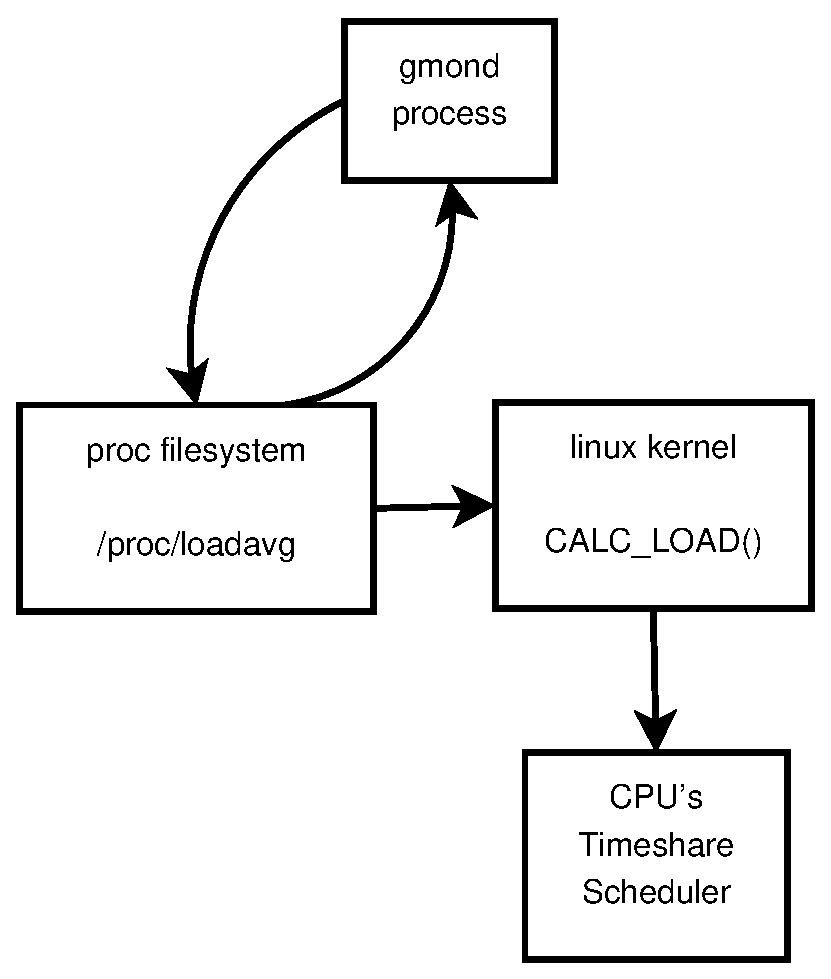
\includegraphics[width=3in]{images/calc_load.eps}
\caption{Load Average calculation}
\label{figure:calc_load}
\end{figure}


\subsection{Ganglia}

The metrics about load in one, five and fifteen minutes are taken from Gmond daemon through the proc filesystem as seen in Figure \ref{figure:calc_load}. These values are multicasted using a UDP message on the network, only if the value has been changed from the previous one taken. There is also a time thresohold that after that time the value is been sent again, even if it haven't changed, so new hosts on the network may gather the data needed for their Gmond. Each host of a cluster have the information about the metrics of itself and each other node, so it stores the whole cluster state. Using loopback interface, every Gmond sends its metrics to itself.

If a TCP connection on the Gmond listening port 8649 is made, Gmond writes a full cluster state of metrics in XML including its DTD. There is a typical access list in the configuration called trusted hosts, and of course every node that is in the cluster that a specific node is configured to be part of, is allowed to connect to get the XML.

\begin{figure}[htb]
\centering
 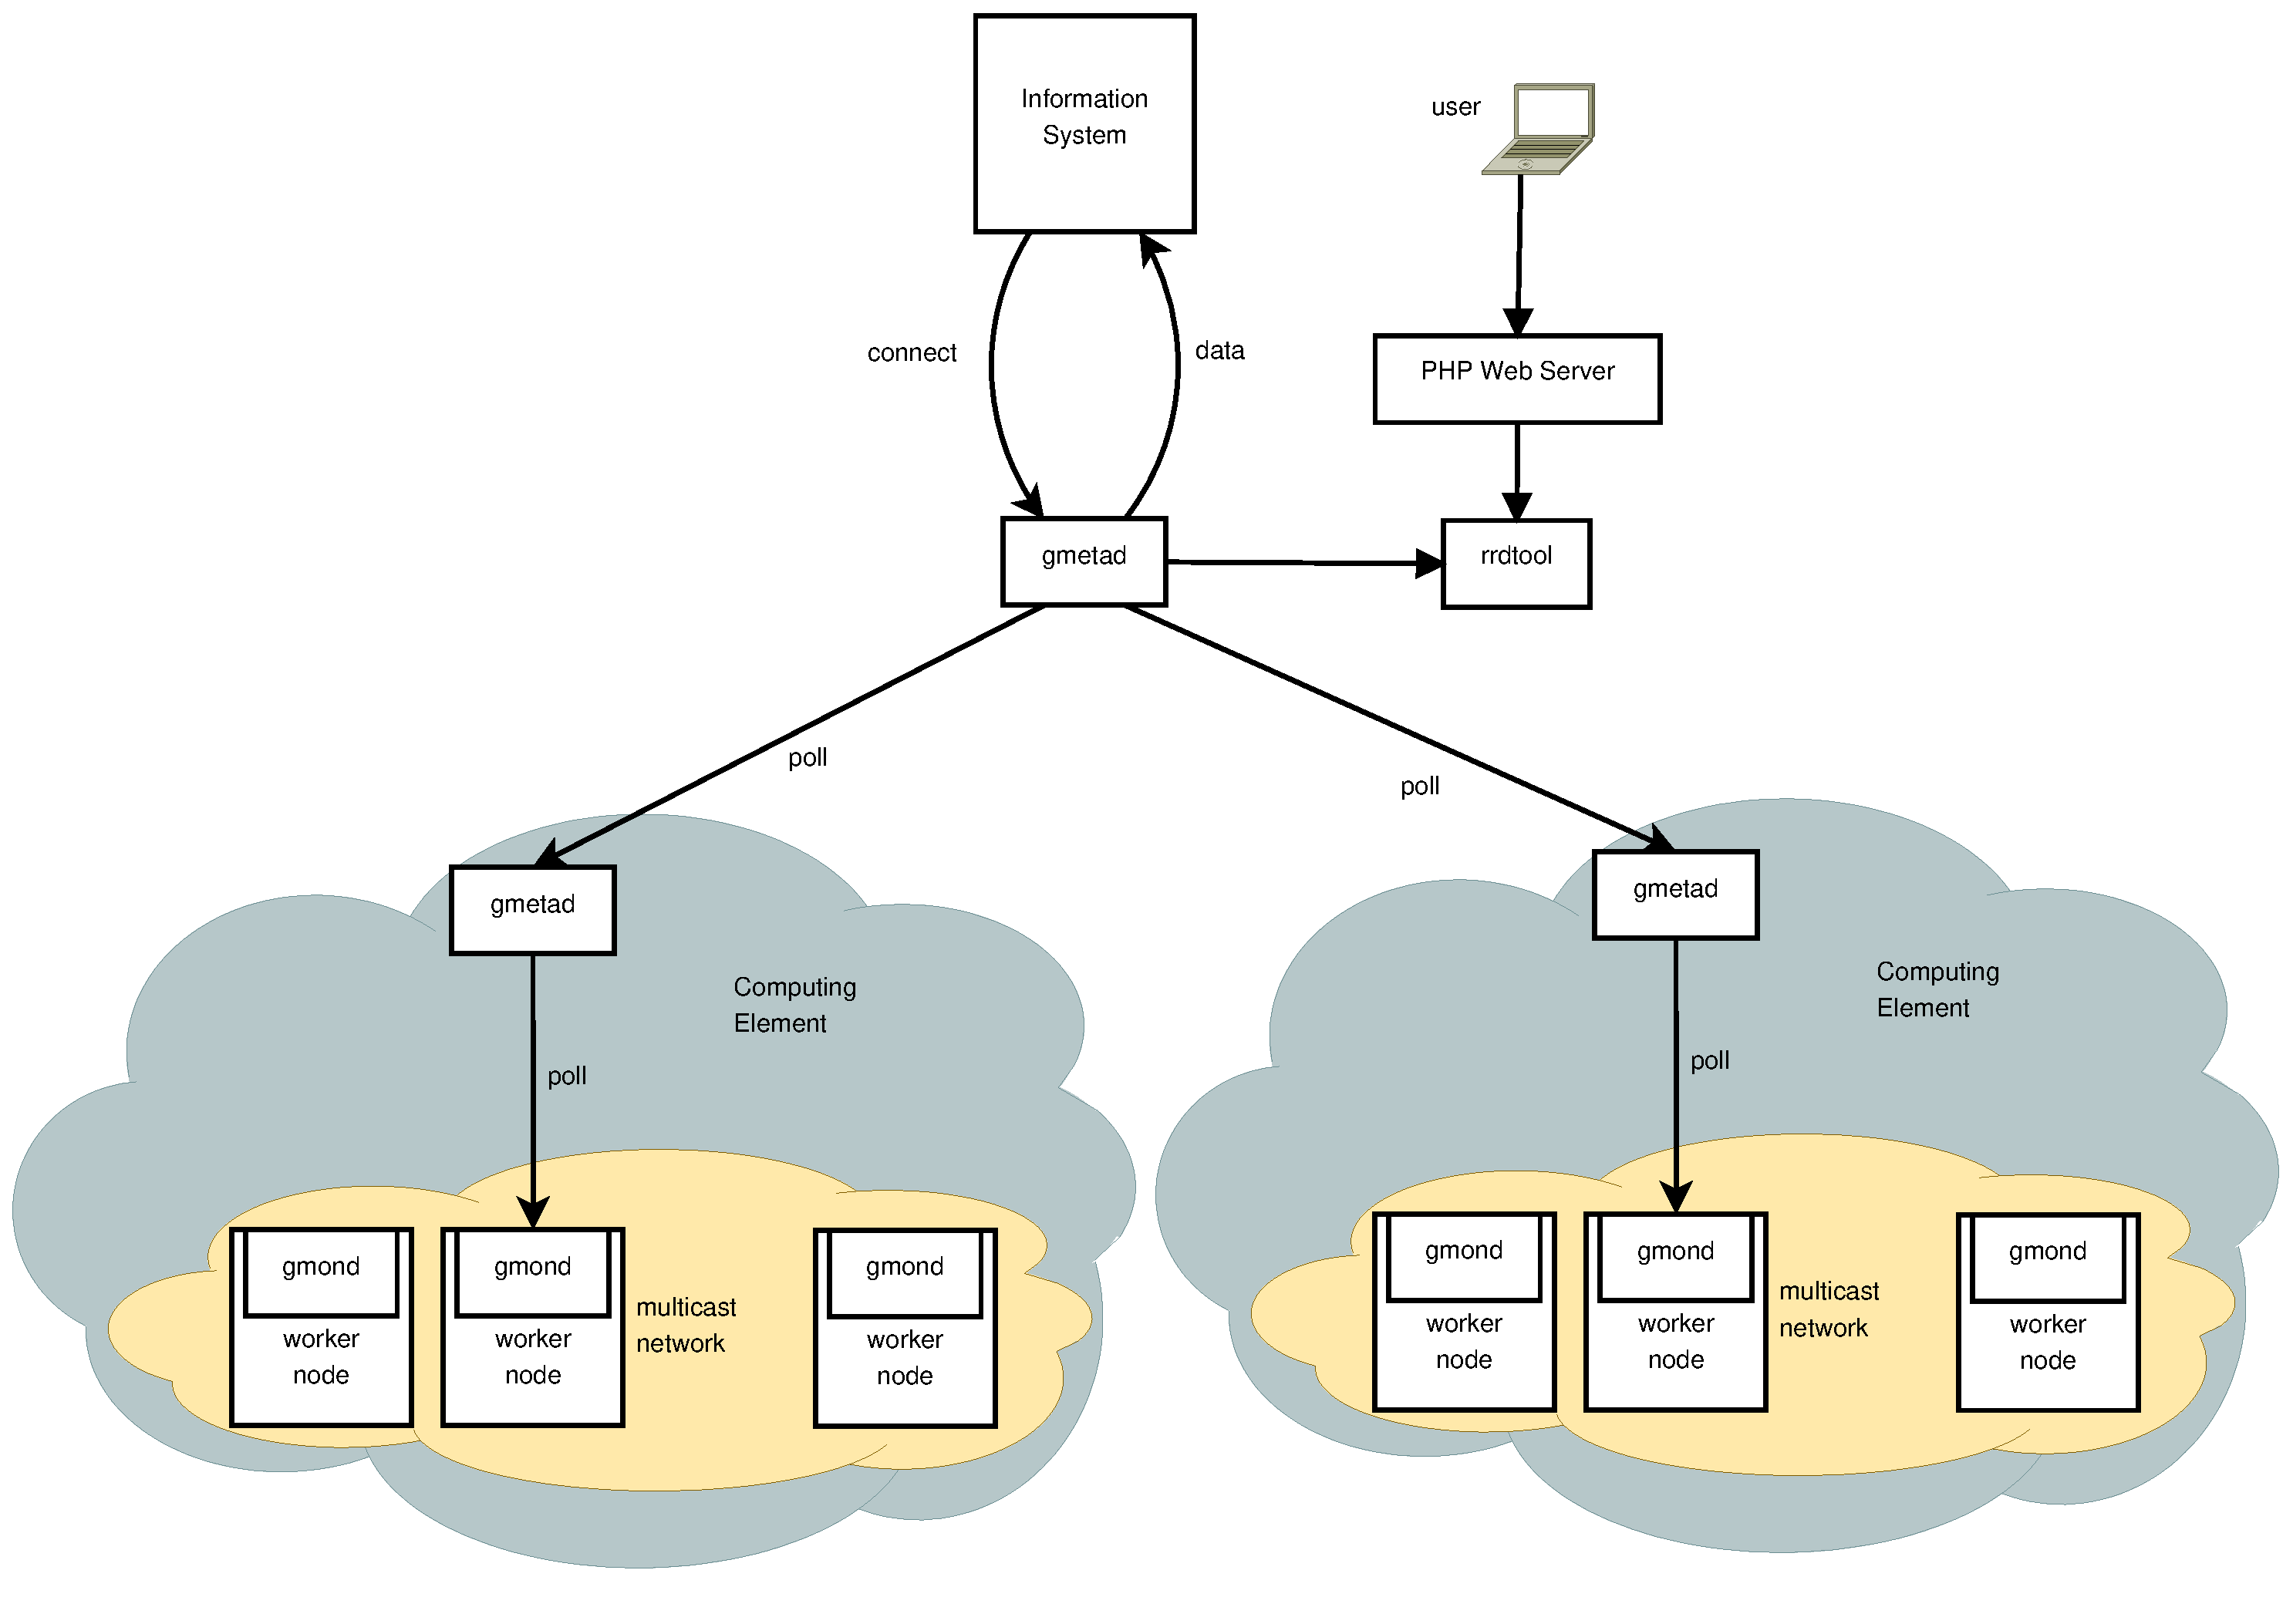
\includegraphics[width=6in]{images/ganglia_data_flow.eps}
\caption{Ganglia Network Communications}
\label{figure:ganglia_network}
\end{figure}



\subsection{Nagios}

Nagios is the core monitoring tool that is used for grid computing monitoring as Multi Level Monitoring architecture proposes, to meet the needs of EGEE/EGI. Following SAM and Gridview, Nagios instances have been deployed in many levels of grid infrastructure, enhansing the functionality of scheduling and execution of site tests. The message bus that uses is MSG, which offers an integration between Nagios and the other monitoring tools of grid.

CERN provides MSG-Nagios-bridge, a mechanism to transfer test results between different levels of Nagios deployment (regional, project, site). MSG-Nagios-bridge both submit tests to other Nagios installations and consume results from them. 

A Regional Metric Store is also used by nagios. It is a database that provides a backend to Nagios current and historical metrics, and connected with the frontend and the message bridge. The adaptor that provides such functionality called NDOUtils, and may have a MySQL/PorstgreSQL or Oracle backend.

In the front-end, users are allowed to discover the nodes and services provided in the monitoring levels by regions, projects and sites, using cgi scripts that are part of the Nagioc core distribution. Access control between levels of Nagios instances and between users and Nagios installations, is performed using the standard methods of grid, which is GOCDB as described in ATP. User authentication is done by user certificates.


\begin{lstlisting}[language=bash,caption=Ganglia to Nagios script]
#!/bin/bash
if [ ! $1 ]
then
        echo "Please HOST argument"
        echo "ex. ganglia_to_nagios 10.0.0.1"
        exit
fi
/usr/src/redhat/SOURCES/ganglia-python-3.3.0/ganglia.py --host $1 --live | while read host
do
        echo ";$host.oslab.teipir.gr
define host{
        use     gmond-host
        host_name       $host.oslab.teipir.gr
        alias           $host
        address         $host.oslab.teipir.gr
        hostgroups      worker-nodes
}
"
done > /etc/nagios/teipir/hosts.cfg
\end{lstlisting}

\begin{figure}[htb]
\centering
 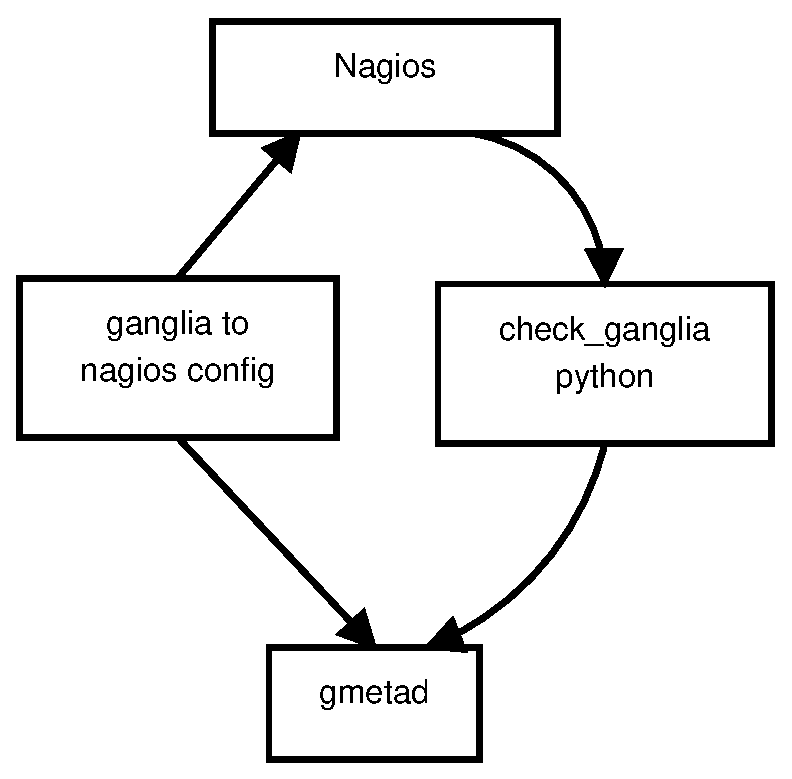
\includegraphics[width=4in]{images/nagios_check_ganglia.eps}
\caption{Nagios configuration and check ganglia values}
\label{figure:nagios_ganglia}
\end{figure}

%TODO some text for NPCD and pnp4nagios
Bulk Mode with NPCD
NPCD:
spool directory to process bulk data
create graphs using RRDTOOL

\begin{figure}[htb]
\centering
 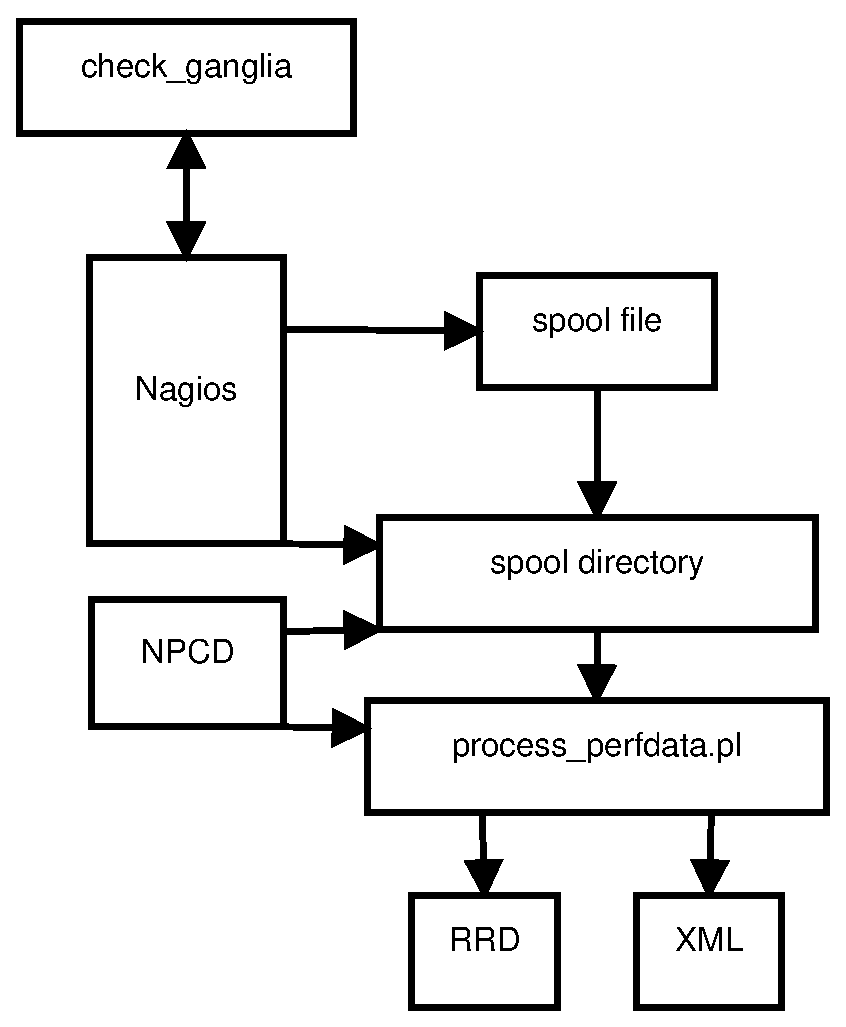
\includegraphics[width=3in]{images/npcd_pnp4nagios.eps}
\caption{PNP 4 Nagios data flow}
\label{figure:pnp4nagios}
\end{figure}

\section{Range of cases examined}

Publish to Information System \cite{goelagent}

\subsection{LDAP based - MDS/BDII}

To integrate Ganglia with MDS in early versions of Globus, there schema of OpenLDAP should be extended using the Glue-CE definitions from the DataTAG web site (MDS version 2.4). A Ganglia Information Provider was the native ganglia client on python, given by the ganglia development team itshelf.

\begin{enumerate}
  \item Python ganglia client script: \url{http://globus.org/toolkit/docs/2.4/mds/gangliaprovider.html}
  \item Perl gaglia-IP tool: \url{http://www.star.bnl.gov/public/comp/Grid/Monitoring/SimpleGangliaIP.html} and \url{http://www.star.bnl.gov/public/comp/Grid/Monitoring/ganglia\_ip}
\end{enumerate}

\begin{verbatim}
# which glue services does the information base provides?
[root@osweb ~]# ldapsearch -h dgc-grid-44.brunel.ac.uk -p 2170 -x -b "mds-vo-name=uki-lt2-brunel,o=grid" '(&(objectclass=glueservice)(GlueServiceType=*))' GlueServiceType |grep "^GlueServiceType" |sort|uniq

# installation of bdii
-install glite-ui which installs bdii
-ldapsearch bdii
-test perl & python scripts to export mds from gmond
-configure connection to 

[root@osweb ~]# /opt/glite/yaim/bin/yaim -c -s site-info.def -n BDII_site

# configure BDII
site-info.def:
# BDII
CE_HOST="osweb.teipir.gr"
SITE_BDII_HOST="osweb.teipir.gr"
SITE_EMAIL="theofpa@teipir.gr"
SITE_LAT=37.979166
SITE_LONG=23.674719
SITE_DESC="TEI of Piraeus"
SITE_LOC="Athens, Greece"
SITE_WEB="http://oslab.teipir.gr"
SITE_SECURITY_EMAIL=$SITE_EMAIL
SITE_SUPPORT_EMAIL=$SITE_EMAIL
SITE_OTHER_GRID="EGEE"
BDII_REGIONS="oslab.teipir.gr"

\end{verbatim}

\begin{table}[ht]
\small\addtolength{\tabcolsep}{-3pt}
\begin{tabular}{ | l | l | r |}
\hline
{\bf Common Name} & {\bf Attribute} & {\bf Objectclass} \\ \hline
Hostname & GlueHostName & GlueHost \\ \hline
Unique ID assigned to the host & GlueHostUniqueID & GlueHost  \\ \hline
Processor Load, 1 Min Average  & GlueHostProcessorLoadLast1Min & GlueHostProcessorLoad \\ \hline
Processor Load, 5 Min Average  & GlueHostProcessorLoadLast5Min & GlueHostProcessorLoad \\ \hline
Processor Load, 15 Min Average  & GlueHostProcessorLoadLast15Min & GlueHostProcessorLoad \\ \hline
SMP Load, 1 Min Average  & GlueHostSMPLoadLast1Min & GlueHostSMPLoad \\ \hline
SMP Load, 5 Min Average  & GlueHostSMPLoadLast5Min & GlueHostSMPLoad \\ \hline
SMP Load, 15 Min Average  & GlueHostSMPLoadLast15Min & GlueHostSMPLoad \\ \hline
Number of CPUs  & GlueHostArchitectureSMPSize & GlueHostArchitecture \\ \hline
Processor Clock Speed (MHz)  & GlueHostProcessorClockSpeed & GlueHostProcessor \\ \hline
Network Interface name  & GlueHostNetworkAdapterName & GlueHostNetworkAdapter \\ \hline
Network Adapter IP address  & GlueHostNetworkAdapterIPAddress & GlueHostNetworkAdapter \\ \hline
The amount of RAM  & GlueHostMainMemoryRAMSize & GlueHostMainMemory \\ \hline
Free RAM (in KBytes)  & GlueHostMainMemoryRAMAvailable & GlueHostMainMemory \\ \hline
\end{tabular}
\caption{GLUE schema for Host Processor Information Provider}
\label{tab:glue}
\end{table}

Perl:
\begin{lstlisting}
$[root@mon ~]# ./ganglia_ip -h mon -p 8649 -o mds
\end{lstlisting}

Python:
\begin{lstlisting}
$[root@mon ~]# /opt/ganglia/bin/ganglia --format=MDS
\end{lstlisting}

\begin{lstlisting}

[root@osweb ~]# cat /opt/glite/etc/gip/provider/glite-info-provider-service-ganglia-wrapper
#!/bin/bash
/opt/bin/ganglia_ip -h 195.251.70.54 -p 8649 -o mds
\end{lstlisting}

\subsection{Web Service based - WSRF}

\subsubsection{container}
using WSRF (GT4, information services, information providers)
Ganglia Resource Provider
MDS Index Service
GLUE CE 

OASIS standard

container
\begin{figure}[htb]
\centering
 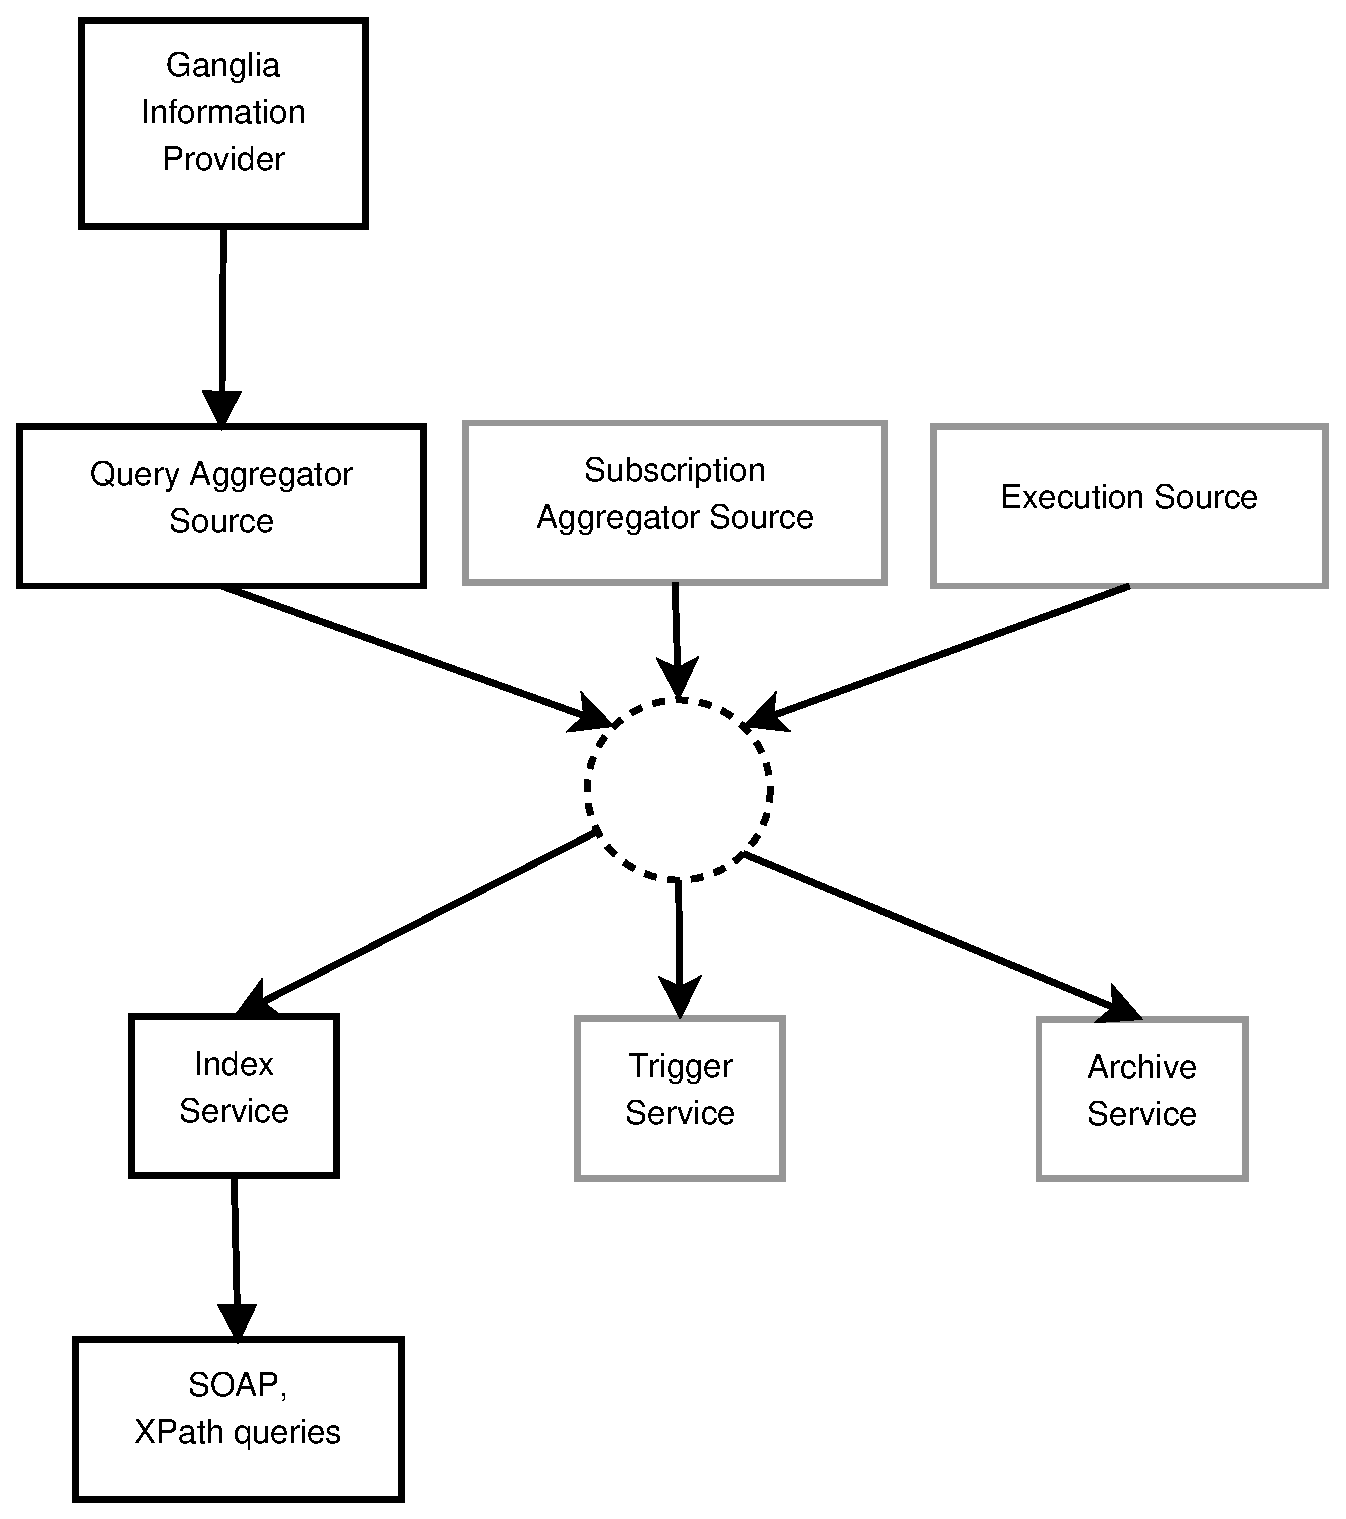
\includegraphics[width=5in]{images/wsrf.eps}
\caption{Web Service Resource Framework}
\label{figure:wsrf}
\end{figure}

\subsection{information provider}

wssd

and

rp xml

and

hierarchy.xml maybe in an "aggregation" section

and

deserialization of MDS query in gmond to WSRF
 
\begin{verbatim}
# installation of globus, wsrf, ganglia:
-download binary 4.0.7 and extract to /opt/globus
wget http://www-unix.globus.org/ftppub/gt4/4.0/4.0.7/installers/bin/gt4.0.7-x86_rhas_4-installer.tar.gz
export $JAVA_HOME=/usr/java/default
[root@osweb ~]# export JAVA_HOME=/etc/alternatives/java_sdk
export PATH=$JAVA_HOME/bin:$PATH
./configure
make
make install
-install postgresql, create user & db
-configure globus to connect to postgresql
-create init script for wsrf container
-create ganglia resource provider for wsrf and connect to gmond
-call wsrf to get ganglia metrics

# query WSRF for ganglia data:
[root@osweb ~]# grid-proxy-init -verify -debug
[root@osweb ~]# wsrf-query -s https://osweb.teipir.gr:8443/wsrf/services/DefaultIndexService "//*[local-name()='Host']"
[root@osweb ~]# /opt/globus/bin/wsrf-query -s https://osweb.teipir.gr:8443/wsrf/services/DefaultIndexService "//glue:Host[glue:ProcessorLoad[@glue:Last15Min>20]]"  |grep Load
\end{verbatim}

\subsubsection{XPath}

XPath is used to parse an XML document and get a part of it using an address scheme. For XPath, the XML document is a tree consisting of nodes, and its purpose as a language is to get the nodes that are addressed using the XPath query from that document.

Its syntax is compact, non-XML and much like the filesystem addressing, so it facilitates the use of XPath within URIs.

Example queries used in this project are:

The following is used in the PHP code that queries the WebMDS for all nodes of the XML of the WSRF containing nodes with name $Host$:
\begin{verbatim}
//*[local-name()='Host']
\end{verbatim}

Another example is a more complex query that asks the WSRF for all nodes with name $Host$ that contains a sub-node named $ProcessorLoad$ and its $Last15Min$ attribute has value larger than 20:
\begin{verbatim}
//glue:Host[glue:ProcessorLoad[@glue:Last15Min>20]]
\end{verbatim}

Finally the following example may return only the $ProcessorLoad$ node of the $Host$ that has the attribute Name set to $xenia.oslab.teipir.gr$:
\begin{verbatim}
//glue:Host[@glue:Name='xenia.oslab.teipir.gr']/glue:ProcessorLoad
\end{verbatim}


\subsubsection{XSLT}

my note: WSRF is GLUE 2.0 schema CE compatible

\begin{verbatim}
file /opt/globus/etc/globus_wsrf_mds_usefulrp/ganglia_to_glue.xslt
\end{verbatim}

\begin{lstlisting}[language=XML,caption=WSRF XSLT for Ganglia Information Provider]
<glue:ProcessorLoad>

<xsl:attribute name="glue:Last1Min">
  <xsl:call-template name="emitProperNumeric">
    <xsl:with-param name="numeric" 
    select="floor(100 * METRIC[@NAME='load_one']/@VAL)"/>
  </xsl:call-template>
</xsl:attribute>

<xsl:attribute name="glue:Last5Min">
  <xsl:call-template name="emitProperNumeric">
    <xsl:with-param name="numeric" 
    select="floor(100 * METRIC[@NAME='load_five']/@VAL)"/>
  </xsl:call-template>
</xsl:attribute>

<xsl:attribute name="glue:Last15Min">
  <xsl:call-template name="emitProperNumeric">
    <xsl:with-param name="numeric" 
    select="floor(100 * METRIC[@NAME='load_fifteen']/@VAL)"/>
  </xsl:call-template>
</xsl:attribute>

</glue:ProcessorLoad>
\end{lstlisting}

\subsubsection{WebMDS}

WebMDS is a web interface to query WSRF resource property information. It consists of forms and views of raw XML or organized in tables of results. This user friendly frontend comes as a part of Globus Toolkit version 4 and it can deployed in any application server. Behind this application reside the data that the WSRF aggregation framework provides through the Index Service.

\begin{figure}[htb]
\centering
 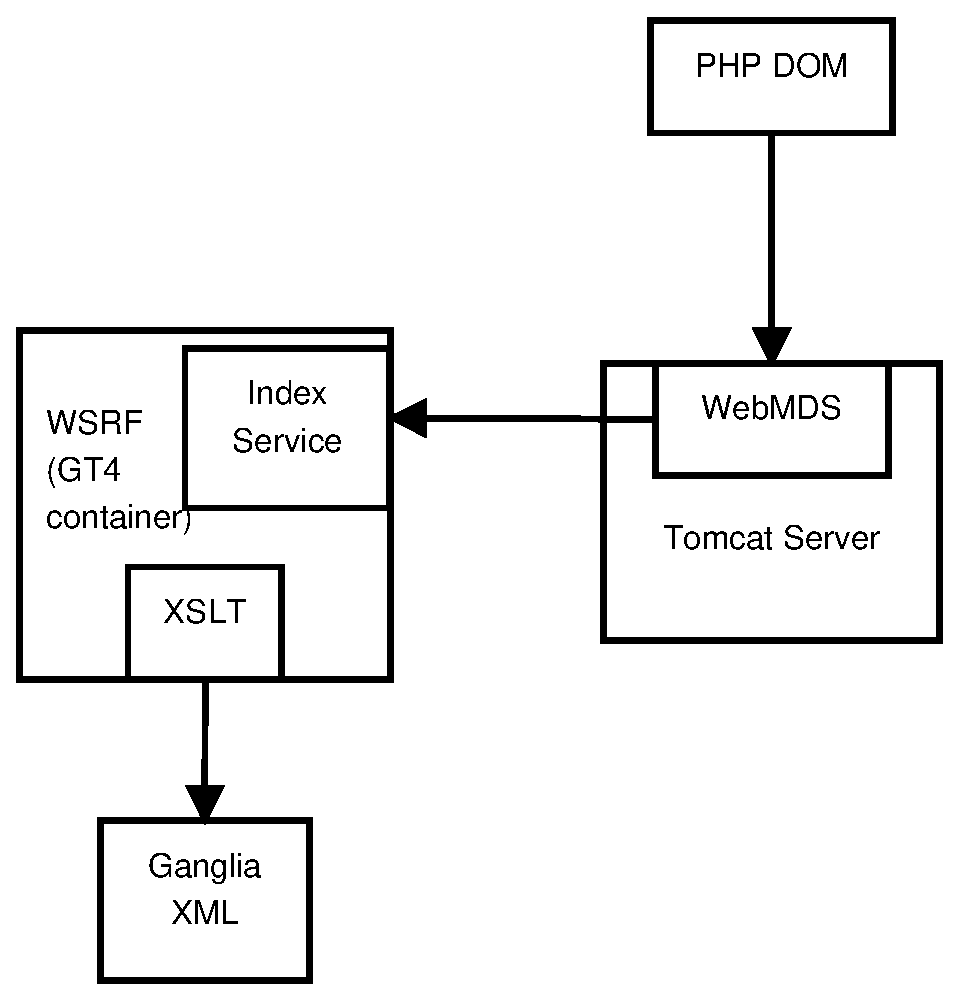
\includegraphics[width=4in]{images/webmds.eps}
\caption{WebMDS application}
\label{figure:webmds}
\end{figure}

For this project an Apache Tomcat server was installed in the box that globus toolkit was running, and the {\bf webmds application} from the GT4 home was deployed. In webmds configuration file, the globa option to allow user specified queries using XPath was enabled.
